\section{La classe NP}
\subsection{Giochiamo a Domino}
Disponete in file le \g{tessere del domino} che vi sono state consegnate in modo da 
usare tutte le tessere. 
% immagine
\g{È un problema facile o difficile da risolvere?}
\begin{definition}
  Un problema è \g{trattabile} (facile) se esiste un \g{algoritmo efficiente}
  per risolverlo
\end{definition}
\begin{itemize}
  \item Gli algoritmi efficienti sono \g{algoritmi con complessità polinomiale}, 
    il loro tempo di esecuzione è $O(n^2)$ per qualche costante $k$.
  \item Avere complessità polinomiale è una \g{condizione minima} per considerare 
    un algoritmo efficiente
  \item Un algoritmo con complessità più che polinomiale (per esempio esponenziale)
    è un algoritmo \g{non efficiente} perché non è scalabile. 
\end{itemize}
\subsection{Mostriamo che Domino[1] è trattabile}
\paragraph{Obiettivo} Trovare un algoritmo polinomiale per \g{Domino[1]}
\begin{itemize}
  \item Formulazione del problema in termini di \g{linguaggio}
  \item Definizione di una Macchina di Turing che lo \g{decide}
  \item Analisi di \g{complessità} della macchina di Turing
    (o dell'algoritmo)
\end{itemize}
\subsection{Un linguaggio e una riduzione}
$D_1=\{\langle B\rangle\mid B\textrm{ 
  è un insieme di tessere del domino, ed esiste un allineamento 
  che usa tutte le tessere
  }\}$
\begin{itemize}
  \item Usiamo una \g{Riduzione mediante funzione} per trovare l'algoritmo
    polinomiale.
  \item Riduciamo $D_1$ ad un \g{problema su grafi}
  \item ... per il quale sappiamo che \g{esiste un algoritmo polinomiale}
\end{itemize}
\subsection{Dalle tessere al grafo}
\begin{definition}
  Un grafo (non orientato) è una coppia (V,E) dove:
 \begin{itemize}
   \item $V = \{v_1, v_2,\dots,v_n\}$ è un insieme finito e non vuoto di \g{vertici}
   \item $E\subseteq\big\{\{u,v\}\mid u,v\in V\big\}$ è un insieme di 
     \g{coppie non ordinate}
     ognuna delle quai corrisponde ad un \g{arco} del grafo.
 \end{itemize} 
\end{definition}
\paragraph{Grafo del dominio}
\begin{itemize}
  \item \g{Vertici}: i numeri che si trovano sulle tessere
    \begin{itemize}
      \item $V = \{\epsdice{1},\epsdice{2},\epsdice{3},\epsdice{4}\}$
    \end{itemize}
  \item \g{Archi}: le tessere del domino
    \begin{itemize}
      \item $E =  \{\epsdice{3}\epsdice{4}, \epsdice{1}\epsdice{2},
        \epsdice{4} \epsdice{2},\epsdice{4} \epsdice{1}, 
                   \epsdice{3} \epsdice{2} \}$
    \end{itemize}
\end{itemize}
\subsection{Dominio[1] è un problema su grafi!}
\g{Camino Euleriamo}: percorso di un grafo che attraversa \g{tutti gli archi}
una sola volta.
\paragraph{Il problema del Cammino Euleriano}
\[
  EULER = \{\langle G\rangle\mid \textrm{
    è un grafo che possiede un cammino Euleriano
  }\}
\]
\begin{itemize}
  \item $EULER$ è un problema classico di \g{teoria dei grafi}
  \item Esistono \g{algoritmo polinomiali} per risolverlo.
\end{itemize}
\subsection{Algoritmo di Fleury}
\begin{itemize}
  \item Scegliere un vertice con \g{grado dispari} 
    (un vertice qualsiasi se tutti pari)
  \item Scegliere un arco tale che la sua cancellazione \g{non sconnetta il grafo}
  \item \g{Passare} al vertice nell'altra estremità dell'arco scelto.
  \item \g{Cancellare} l'arco del grafo
  \item \g{Ripetere} i tre precedenti finché non eliminate tutti gli archi
\end{itemize}
\paragraph{Complessità} Su un grafo con $n$ archi, l'algoritmo di Fleury impiega 
tempo $O(n^2)$ 
\subsection{Complessità di Domino[1]}
\begin{itemize}
  \item L'algoritmo di Fleury risolve $EULER$ in tempo \g{polinomiale}
  \item La riduzione ci dice che $D_1 \leq_m EULER$ 
  \item Quanto tempo serve per risolvere il problema $D_1$? 
\end{itemize}
\subsection{Giochiamo a domino[2]}
Disponete in file le tessere del domino che vi sono state consegnate in modo che 
\g{ogni numero} compaia \g{esattamente due volte}
(potete usare meno tessere di quelle che avete)
\g{È un problema facile o difficile da risolvere?}
\subsubsection{Una riduzione in senso opposto!}
\[
  D_2 = \{\langle B\rangle\mid B\textrm{ insieme di tessere del domino, ed } \exists 
 \textrm{ allineamento dove ogni numero compare 2 volte}\}
\]
\begin{itemize}
  \item \g{Corcuito Hamiltoniano}: ciclo nel grafo che attraversa \g{tutti i vertici}
    una sola volta
\end{itemize}
\begin{definition}[Il problema del Circuito Hamiltoniano]
  $HAMILTON =\{\langle G\rangle\mid G\textrm{ è un grafo con un circuito Hamiltoniano}\}$
\end{definition}
Come facciamo a dinostrare che $HAMILTON \leq_m D_2$? 
\subsection{$HAMILTON$ è un problema difficile!}
\begin{itemize}
  \item Il problema del \g{circuito Hamiltoniano} è un problema classico di 
    \g{teoria dei grafi}
  \item Un \g{algoritmo polinomiale} per risolverlo \g{non è mai stato trovato}
  \item Se qualcuno mi dà una \g{possibile soluzione}, è \g{facile verificare} 
    se è corretta
\end{itemize}
\subsection{Problemi trattabili e probemi intrattabili}
\begin{itemize}
  \item I problemi per i quali esiste un algoritmo polinomiale vengono considerati
    \g{trattabili}
  \item quelli che richiedono un algoritmo più che polinomiale sono detti \g{intrattabili}
  \item Sappiamo che ci sono problemi che non possono essere risolti da \g{nessun algoritmo}:
    \begin{itemize}
      \item ``Hamilton Problem'' di Turing.
    \end{itemize}
  \item Ci sono problemi che richiedono un tempo \g{esponenziale}
    \begin{itemize}
      \item Il gioco della Torre di Hanoi
    \end{itemize}
\end{itemize}
\begin{center}
  \g{Stabilire con precisione qual'è il confine tra problemi trattabili 
  ed intrattabili è piuttosto difficile} 
\end{center}
\subsection{P vs NP}
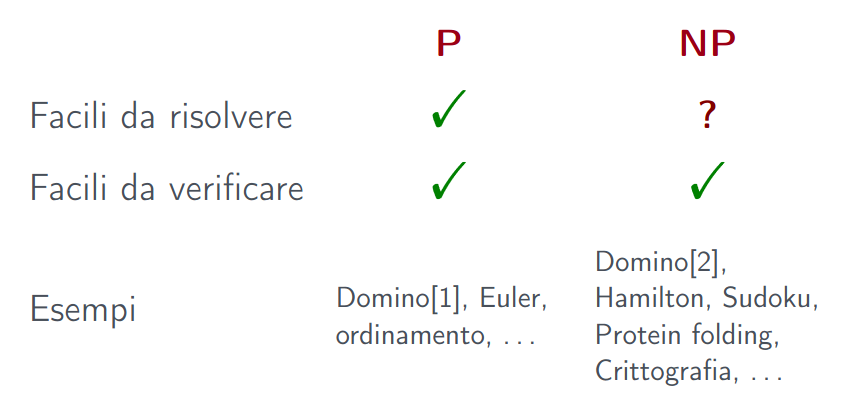
\includegraphics[scale=0.5]{img/pvsnp.png}

% SCHIFEZZE DELLA ISSUE #34 DI GITHUB

\subsection{Verificatori}
\begin{definition}
  Un \g{verificatore} per il linguaggio $A$ è un algoritmo $V$ tale che 
  \begin{displaymath}
    A+\{w\mid V\textrm{ accetta } \langle w,c\rangle\textrm{ per qualche stringa }c\}
  \end{displaymath}
\end{definition}
\begin{itemize}
  \item Il verificatore usa \g{ulteriori informazioni} per stabilire se $w$ appartiene 
    al linguaggio
  \item questa informazione è il \g{certificato} c
\end{itemize}
\subsection{Problemi P ed NP} 
\begin{description}
  \item [P] è la classe dei linguaggi che possono essere \g{decisi} da una 
    macchina di Turing deterministica che inpiega \g{tempo polinomiale}
  \item [NP] è la classe dei linguaggi che ammettono un \g{verificatore}
    che impiega \g{tempo polinomiale}
  \item [Equivalente] è la classe dei linguaggi che possono essere decisi da una macchina 
    di Turing \g{non deterministica} che impiega \g{tempo polinomiale}.
\end{description}
\subsubsection{Due problemi in P}
\paragraph{Raggiungibilità di un grafo}\nin

$PATH=\{\langle G,s,t\rangle\mid G \textrm{ grafo che contiene un cammino da } s \textrm{ a }t\}$
\paragraph{Numeri relativamente primi}\nin

$RELPRIME = \{\langle x,y\rangle\mid 1 \textrm{ è il massimo comun divisore di }x\textrm{ e }y\}$
\subsubsection{Due problemi in NP}
\paragraph{Problema del circuito Hamiltoniano}\nin

$HAMILTON =\{\langle G\rangle\mid G\textrm{ è un grafo con un circuito Hamiltoniano}\}$
\paragraph{Numeri composti}\nin

$COMPOSITES = \{\langle x\rangle\mid x = pq\textrm{, per gli interi }p,q>1\}$
